
\documentclass[12pt]{amsart}


% Language
\usepackage[utf8]{inputenc}
% Math
\usepackage{amsmath}
\usepackage{amssymb}
\usepackage{fancyvrb}
% Drawing
\usepackage{tikz}
\usepackage{graphicx}
% Lists
\usepackage{listings}
\usepackage{subcaption}
% Source code
\usepackage{verbatim}

% USER DEFINED


% Positioning

%% Frame around everything
%%\usepackage[showframe,textwidth=3.0in]{geometry}
\usepackage[textwidth=6.5in]{geometry}
%% The rest (position):
\usepackage{xstring}% for string comparrison
\usepackage{calc}%    for \widthof
\usepackage{pgf}%     for math calclations
%%% Positioning command
\newlength{\Size}
\newcommand*{\PositionText}[3][l]{%
    \IfStrEqCase{#1}{%
        {l}{\noindent\hspace{#2}#3}%
        {c}{\pgfmathsetlength{\Size}{#2-0.5*(\widthof{#3})}\noindent\hspace{\Size}#3}%
        {r}{\pgfmathsetlength{\Size}{#2-1.0*(\widthof{#3})}\noindent\hspace{\Size}#3}%
        }[\PackageError{PositionText}
            {\MessageBreak Unrecognized alignment: #1.\MessageBreak 
            Valid alignments are are `l`, `c`, `r'}{}]%
}%


% Drawing
\usepackage[usenames,dvipsnames]{pstricks}
\usepackage{epsfig}
\usepackage{pst-grad} % For gradients
\usepackage{pst-plot} % For axes

% Remove unicode space
\DeclareUnicodeCharacter{00A0}{ }

% User defined commands

\newcommand{\party}[2]{\frac{\partial #1}{\partial #2}} %
\renewcommand{\d}{\mathrm{d}}
\renewcommand{\b}[1]{\textbf{#1}}
\newcommand{\exer}[1]{\noindent \textbf{#1}} 
\newcommand{\eps}{\varepsilon}
\newcommand{\s}{\sigma}
\newcommand{\p }{\partial }
\newcommand{\del }{\nabla}

% User defined colors
\definecolor{myblue}{rgb}{0.3,0.3,1}
\definecolor{mygray}{rgb}{0.4,0.4,0.4}
\definecolor{mygray2}{rgb}{0.98,0.98,0.98}

% Source code settings
\lstset{keywordstyle=\color{myblue},backgroundcolor=\color{mygray2},basicstyle=\footnotesize\ttfamily,breaklines=true,commentstyle=\color{mygray},language=Python,firstline=1,lastline=53,frame=single,numbers=left,numberstyle=\tiny\color{mygray}}

% Title ++
\title{MEK 4300\\Mandatory assignment 1}	
\author{Henrik Aasen Kjeldsberg}
\date{\today}
\begin{document}
\maketitle
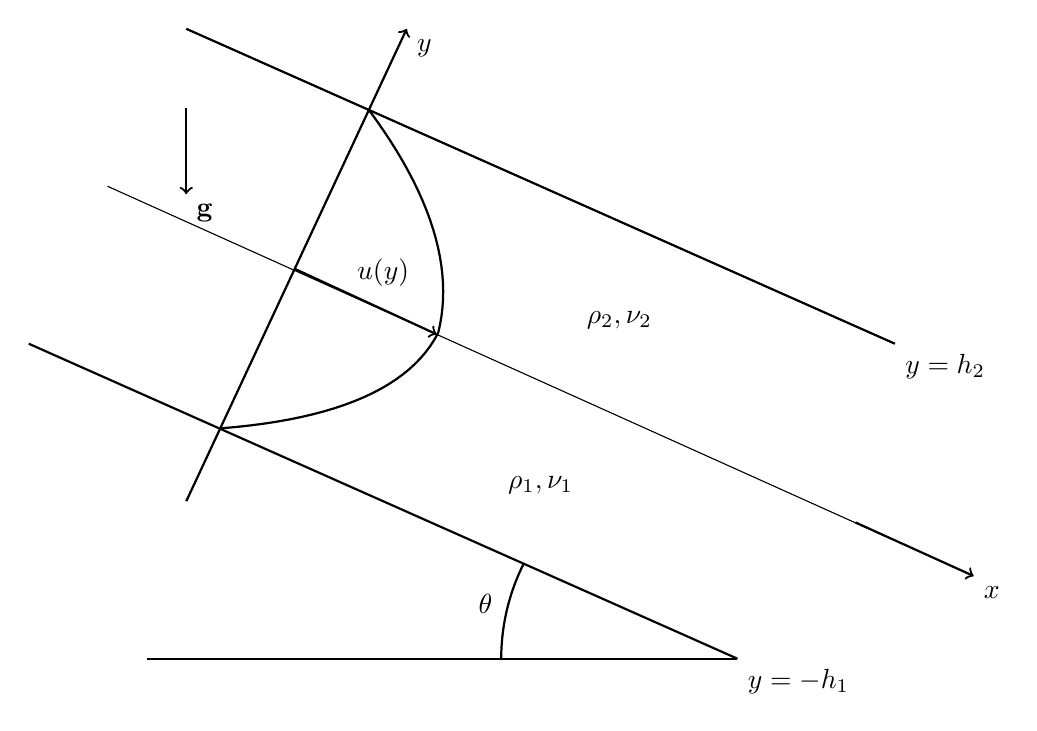
\begin{tikzpicture}
  \draw[thick] (-2.5,6) -- (6.5,2) node[anchor=north west] {$y=h_2$};
  \draw (-3.5,4) -- (6.5,-0.5);
  \draw[thick] (-4.5,2) -- (4.5,-2) node[anchor=north west] {$y=-h_1$};
  \draw[thick] (-3,-2) -- (4.5,-2);
  \draw[thick] (1.5,-2) arc (-180:-206.5:2.7cm);
  \draw[thick,->] (6,-0.27) -- (7.5,-0.95) node[anchor=north west] {$x$};
  \draw[thick,->] (-2.5,0) -- (0.3,6) node[anchor=north west] {$y$};
  \draw[thick,->] (-2.5,5) -- (-2.5,3.9) node[anchor=north west] {$\b g$};
  \draw[thick,->] (-1.12,2.95) -- (0.68,2.12) ;
  \draw (1.3,-1.3) node {$\theta$};
  \draw (0.0,2.9) node {$u(y)$};

  \draw (3.0,2.3) node {$\rho_2, \nu_2$};
  \draw (2.0,0.2) node {$\rho_1, \nu_1$};

  \begin{scope}[shift={(0.7,2.14)}]
  \draw[thick, rotate=76, domain=0:2.53] plot ({\x},{0.24*\x*\x});
  \draw[thick, rotate=63, domain=-2.33:0] plot ({\x},{0.35*\x*\x});
  \end{scope}
\end{tikzpicture}

\begin{tikzpicture}
  \draw[thick] (-2.5,6) -- (6.5,2) node[anchor=north west] {$y=h$};
  \draw[thick] (-4.5,2) -- (4.5,-2) node[anchor=north west] {$y=-h$};
  \draw[thick] (-3,-2) -- (4.5,-2);
  \draw[thick] (1.5,-2) arc (-180:-206.5:2.7cm);
  \draw[thick,->] (5,0.3) -- (7.5,-0.8) node[anchor=north west] {$x$};
  \draw[thick,->] (-2.5,0) -- (0.3,6) node[anchor=north west] {$y$};
  \draw[thick,->] (-2.5,5) -- (-2.5,3.9) node[anchor=north west] {$\b g$};
  \draw[thick,->] (-1.12,3) -- (0.68,2.15) ;
  \draw (1.3,-1.3) node {$\theta$};
  \draw (0.0,2.9) node {$u(y)$};

  \draw (3.0,1.3) node {$\rho, \nu$};

  \begin{scope}[shift={(0.7,2.14)}]
  \draw[thick, rotate=66, domain=-2.25:2.23] plot ({\x},{0.4*\x*\x});
  \end{scope}
\end{tikzpicture}
\end{document}
